\documentclass[conference]{IEEEtran}
\IEEEoverridecommandlockouts
% The preceding line is only needed to identify funding in the first footnote. If that is unneeded, please comment it out.
\usepackage{cite}
\usepackage{amsmath,amssymb,amsfonts}
\usepackage{algorithmic}
\usepackage{graphicx}
\usepackage{textcomp}
\usepackage{xcolor}
\def\BibTeX{{\rm B\kern-.05em{\sc i\kern-.025em b}\kern-.08em
    T\kern-.1667em\lower.7ex\hbox{E}\kern-.125emX}}
\begin{document}

\title{Dynamic Memory Optimization of Serverless Functions using Reinforcement Learning\\

}

\author{
    \IEEEauthorblockN{Hao Zhang}
    \IEEEauthorblockA{haoz18@illinois.edu}
    \and
    \IEEEauthorblockN{Yunxuan Li}
    \IEEEauthorblockA{yunxuan6@illinois.edu}
    \and
    \IEEEauthorblockN{Cesar Arevalo}
    \IEEEauthorblockA{cesara2@illinois.edu}
    \and
    \IEEEauthorblockN{Bingzhe Liu}
    \IEEEauthorblockA{bingzhe@illinois.edu}
    \and
    \IEEEauthorblockN{Reza Farivar}
    \IEEEauthorblockA{farivar2@illinois.edu}
}

\maketitle

\begin{abstract}
Serverless functions have undergone increasing adoption over the past years because of its flexibility, scalability, and ease of use. While users no longer have to deal with the deployment, scheduling or lower-level resource provisioning, memory still remains to be configured properly. Moreover, performance of a serverless function could largely vary as the pattern of incoming requests changes. It continues to be a challenge to find the best memory size to fulfill an optimization objective dynamically. 

In this paper we introduce a framework which adopts reinforcement learning, specifically the contextual multi-armed bandit, to dynamically learn and find the optimal memory configuration for a target serverless function in order to optimize a user-specified objective like time or budget. We evaluated our framework using different types of serverless functions, and our results on synthetic applications show that the framework are effective at single objective, but not practical at composite objectives.
\end{abstract}

\begin{IEEEkeywords}
serverless function, dynamic resource allocation, multi-armed bandit, reinforcement learning, serverless
\end{IEEEkeywords}

\section{Introduction}
%context
Serverless computing has become a major paradigm of cloud computing, and the market is expected to maintain its growing trend in the upcoming future. Cloud Providers have embraced Function as a Service (FaaS), which provides a serverless execution environment for applications. The cloud providers provide few configuration options that affect FaaS runtime environments, the most important one being the ability to configure the memory size \cite{aws-lambda, 10.1145/3429880.3430094}. While past research has shown that memory size of a FaaS function impacts its function performance greatly \cite{10.1145/3464298.3493398}, it is not trivial to automatically identify the optimal memory configuration that would produce the ideal performance in terms of budget, cost, or other objectives like Service-level objective (SLO). The variability of FaaS function performance worsens this issue \cite{10.1145/3429880.3430099}.

\textbf{Optimization methods} have been explored to learn the optimal behavior of target FaaS functions at runtime. This path requires performance testing, i.e. configuring the target function with different resource settings and observe its performance in production \cite{9155363, 8567674, 9860980, 9460548, 10.1007/978-3-031-04718-3_9}.

\textbf{Machine learning} is another way that has been explored to optimize the resource allocation. Machine learning methods require training a model offline, and deploying it for in-production prediction \cite{10.1145/3464298.3493398}.

\textbf{Cloud Providers} have also developed tools to optimize resource provisioning in their backends \cite{10.1145/3552326.3567496, aws_operating_lambda_performance_optimization}.

In this paper, we implement a framework that can automatically find and apply an optimal resource configuration for a serverless function at runtime, with the adoption of a reinforcement learning algorithm called contextual multi-armed bandit.

Reinforcement learning refers to having an agent learn to pick an optimal behavior given a dynamic environment in order to maximize an objective. A Multi-Armed Bandit (MAB) is a simplified version of a reinforcement learning algorithm, where the environment is stateless, in this case the agent only needs to learn about the user behavior and the corresponding reward in order to pick one arm from all candidate arms to maximize the desired reward.

Vanilla MAB algorithms only use an observed reward to find the optimal arm. However, in certain circumstances, other context of the trial could also influence which arm would lead to the optimal reward. The supplementary details, beyond the reward metric, are referred to as contextual features. Bietti et al. \cite{10.5555/3546258.3546391} provide a systematic overview of how a multi-armed bandit optimizes for a given reward using contextual features. Generally speaking, the supplemental contextual features in MAB involves training a machine learning model inside the MAB agent to predict a reward given the input features, and then adding a layer of explore/exploit strategy on top of the model prediction to generate recommendations. We believe this Contextual Multi-Armed Bandit idea could be further expanded to optimize for resource configurations of FaaS functions, using metrics from the incoming requests, and knowing that different kinds of requests will lead to varying execution times, the metrics can be incorporated as contextual features which could optimize the resource allocation efficiency.
% design

Our proposed framework supports flexible and customizable optimization objective - minimal execution time, minimal cost, or SLO. For a deployed FaaS function, the reinforcement learning agent would explore different configurations at the beginning, observe the feedback and reward at runtime, learn the pattern, and quickly converge to the optimal configuration choice. The framework is capable of finding the optimal resource configuration for various types of FaaS functions, and is able to adapt to different workload patterns dynamically and quickly when input traffic starts to exhibit different behavior, which reflects the need of a new optimal memory configuration. The framework is designed to support optimal memory configuration of AWS lambda function, but we believe this algorithm and workflow can be extended to other FaaS platforms as well.
% evaluation

We evaluate our framework using four different types of synthetic serverless functions with following characteristics: cpu-intensive, memory-intensive, image processing, and big data processing. So far experiments have shown that for all four functions, our framework is able to find the right memory size that optimizes for execution time given input requests with stable or varying patterns.
% contribution

To the best of our knowledge, we are not aware of any previous research that utilizes multi-armed bandit, or more generally, reinforcement learning, and incorporates context features to address resource optimization issues of FaaS functions. Additionally, our framework is the first one that learning at runtime, and optimizes memory dynamically given changing request patterns. Our main contributions are summarized below:

\begin{itemize}
    \item Dynamically and automatically optimize resource configuration given changing traffic patterns
    \item The framework is implemented in AWS and published online, supporting easy adoption
    \item We demonstrates that the framework can accurately and quickly picks the best candidate memory size that optimizes for execution time for synthetic serverless functions.
  %todo for next time: add more details to this section
\end{itemize}

Our work expands and deepens the understanding of dynamic FaaS memory optimization, and we designed a system that is able to optimize memory configuration on different type of functions with single optimization goals. We also discovered some limitations of our system and proposed future improvement.

\section{Background}

Past research has attempted to address the challenges of finding the optimal memory size of serverless functions using different approaches. Resource optimization in the serverless computing domain continues to be an area of active research and development \cite{10.1145/3587249, 10.1145/3406011, 9756233}, because of the constraints imposed to both the users and providers, i.e. memory, CPU, SLO/QoS, cost, scheduling, etc. \cite{10181224, 10.1145/3542929.3563469, 9860980, 9460548, 10.1145/3429880.3430099}. The resource optimization challenge can be categorized as follows, with solutions falling into a mix of these categories, as we will elaborate further:

\begin{enumerate}
    \item Perspective (of the): Users (e.g. FaaS developers); Providers (or FaaS platform)
    \item Use case: General (e.g. any function); application specific (i.e. DL training)
    \item Algorithm training: offline; online; or both
    \item Goal: Performance; cost
    \item Setup: Static (e.g. one-off, startup); Dynamic (e.g. during runtime)
\end{enumerate}

The FaaS Cloud Providers (e.g. AWS, GCP, Azure) are also doing research on resource optimization of their FaaS backends. Palette Load Balancing \cite{10.1145/3552326.3567496} utilizes locality hints for Serverless Functions on Azure, embedding locality as a firs-level concern in a FaaS platform for optimal performance and efficiency. AWS lambda is frequently updating it's service \cite{aws_new} and has sponsored research on cost/performance optimization \cite{aws_operating_lambda_performance_optimization}.

The Lambda Power Tuning Tool by AWS \cite{aws_lambda_power_tuning} has the capability to optimize for either cost or execution time, but it requires a minimum of requests to be made against the lambda function, which can be cost prohibitive or impractical. Our system aims to streamline the tuning process and not require to run the function a lot of times before being able to find an optimization configuration.

FaaS framework research includes Kraken \cite{10.1145/3472883.3486992}, focused on the optimization of container scheduling and provisioning for FaaS in a container environment, while meeting SLOs. Hermod \cite{10.1145/3542929.3563468} researched the optimal scheduling or serverless functions, built on Apache OpenWhisk, it demonstrated significant performance improvements on slowdown and load. Cypress \cite{10.1145/3542929.3563464} developed an algorithm for serverless platforms that handles container provisioning and request scheduling while being input size-sensitive. Manner and Wirtz \cite{9860370} compared commercial and open-source FaaS platforms resource optimization, providing insights into the QoS scaling of resources, providing different outcomes with regards to the linear scaling of performance vs costs.

From a FaaS user perspective, the COSE \cite{9155363} adopts a Bayesian Optimization algorithm to learn and update configuration to measure performance at different resource settings until convergence is reached, in order to find the best configuration that minimizes cost or execution time. Raza et al. \cite{10063937} continued the work on COSE, furthering the research on the use of Bayesian optimization of configuration parameters, with the goals of adhering to SLO requirements and optimizing for cost. However, these solutions do not perform as well under varying input sizes, and there is an overhead to the sampling data required to update the dynamic function parameters.

Research has been done on different FaaS use cases, e.g., single-function \cite{10.1145/3429880.3430099, 9946331, 9881584}, multi-functions applications \cite{s23187829, 8567674} or application specific \cite{9826021} (e.g., Deep learning training). Sizeless \cite{10.1145/3464298.3493398} generates an offline training dataset by building many synthetic applications and collecting their performance data at different resource configurations. It then trains a neural-network model with the training dataset to predict an optimal memory size for a new unseen single function using production monitoring data as features. This method relies heavily on the quality and generalizability of the offline training dataset. Costless \cite {8567674} optimizes for both cost and execution time of multiple functions, constructing a Cost Graph with observed data, identifying when multiple functions could be fused into one, systematically deciding on which functions to fuse, and determining an optimal memory allocation for each function.

SLAM \cite{9860980} optimizes memory of a FaaS application, which consists of serverless functions and models them as a directed acyclic graph (DAG), by first detecting the relationship among the inner FaaS functions, measuring response time of each function, and then iteratively upgrading the resources allocated to the slowest function in iteration, until the end-to-end SLO is met, while also optimizing another objective like execution duration or budget.

Astra \cite{9460548}, derives models to measure cost and execution time, and makes use of graph theory to obtain an optimal job execution plan. Automatically orchestrates and configures serverless analytics jobs (e.g., map/reduce) while taking into account flexibly-specified user requirements (e.g., performance, cost) and multi-dimensional factors (e.g., function memory size, degree of parallelism at each stage), leveraging graph theory (e.g., Djikstra's and DAGs) it finds the optimal job execution, optimizing for either cost and/or time.

MAFF\cite{10.1007/978-3-031-04718-3_9} is a framework developed by Zubko et al. to find the optimal memory of a FaaS function given user-specified objectives (cost or balanced between cost and execution time), using a few developed heuristic optimization methods, such as linearly searching for better memory size, or finding a memory size using binary search.

Ginzburg and Freeman \cite{10.1145/3429880.3430099} demonstrated that the AWS Lambda performance variability is significant, and it is stable enough to exploit, with the conclusion that further optimizations by the cloud provider are still needed. The solutions proposed included delaying and/or scheduling workloads at various times, something that can be impractical for latency critical workloads.

The offline resource optimization algorithms have required either training datasets \cite{10.1145/3464298.3493398, 10.1145/3542929.3563468}, the pre-processing of lambda functions for setup \cite{10.1109/INFOCOM48880.2022.9796962, 8567674}, sampling of functions to obtain profile metrics \cite{10.1145/3542929.3563464}, or function introspection to gauge resource utilization \cite{s23187829, 9336272}. All of these approaches have drawbacks, they either require overhead in time spent obtaining the datasets, have costs incurred on running the sampling functions, or they are using synthetic/artificially generated application metrics.

The online approaches for resource optimizations have used various ways to gather performance metrics (e.g., memory, CPU, etc.). The use of log parsing has been broadly used in cloud providers (e.g., AWS Lambda), to drive algorithms whose outputs drive the reconfiguration of functions \cite{10063937, 9860980}. Similarly, research on FaaS frameworks, e.g. OpenWhisk, OpenFaaS, has been able to leverage a combination of monitoring tools, orchestrator/scheduler logs, and underlying architectures for gathering performance metrics \cite{9582234, 10.1145/3472883.3486992, 9946331}. However, these approaches require significant setup time for obtaining the performance metrics, or they are not used in a dynamic manner to reconfigure the functions automatically.


\section{System Design}

\begin{figure*}
    \centering
    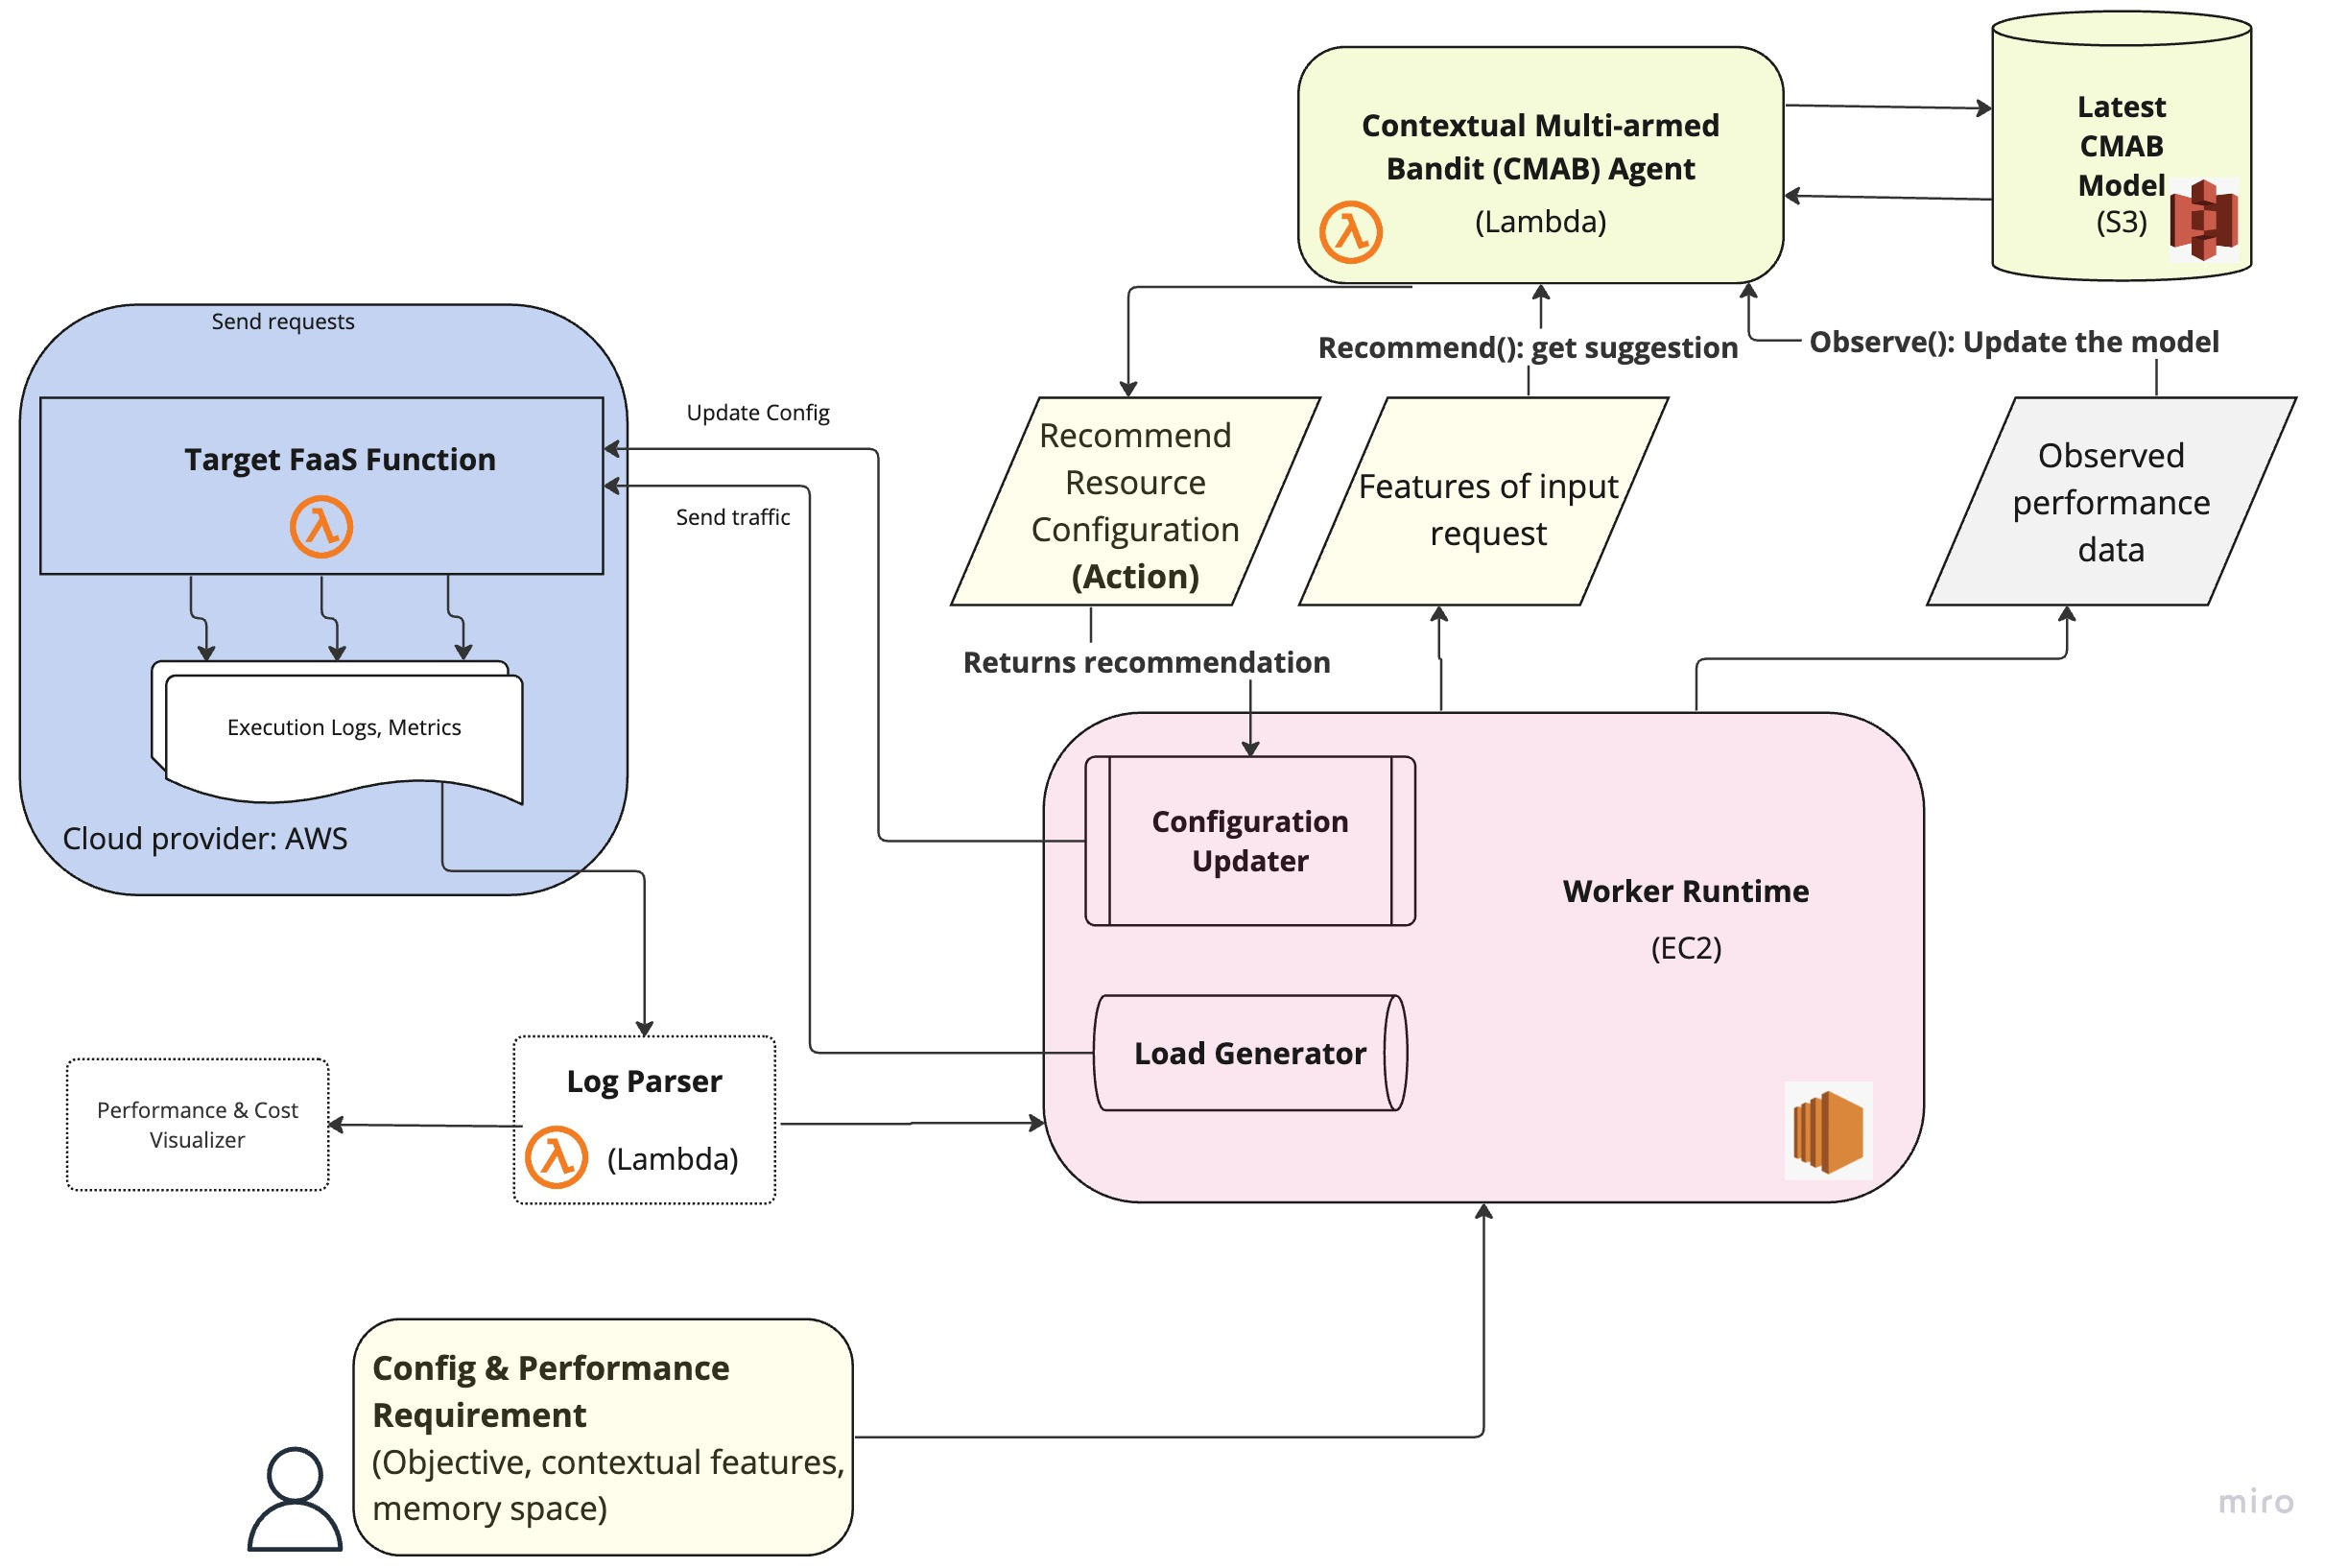
\includegraphics[width=0.75\linewidth]{System Architecture New.PNG}
    \caption{High-level architecture of the system and the interaction
between its components in a general use case}
    \label{fig:enter-label}
\end{figure*}

The latest high-level overview of the system workflow can be found in Figure 1. We implemented our system on Amazon Web Services (AWS), but this framework could easily be expanded to other cloud providers. Our code is available in a github repo (private) \footnote{https://github.com/yunxuanuiuc/Dynamic\_FaaS\_Resource\_Optimization}. 

The framework consists of the following components:

\begin{itemize}

\item CMAB-based Reinforcement Learning Agent (implemented).

The core of the system is a contextual multi-armed bandit (CMAB) agent, a type of reinforcement learning algorithms, which observes historical performance data of the target FaaS function, and makes a recommendation on the ideal memory size for the FaaS function.

The algorithm is implemented using VowpalWabbit \cite{vowpal-wabbit}, an open-source contextual bandit package that supports easy integration of basic CMAB algorithms. The CMAB agent lives in a separate lambda function to support flexible memory optimization requests at any time. Using AWS S3 to store the learned model, because of the stateless nature of lambda functions, and load it to the CMAB agent lambda function when it is triggered.

The CMAB agent requires the basic information of the optimization problem to be set up. We need to pass in the follow information: 
\begin{itemize}
    \item The objective, i.e., the reward to optimize for. Per our problem statement, it supports either "time" or "reward" as objective.
    \item A list of candidate memory sizes. In AWS, the only configurable resource of FaaS functions is memory. Note that here we narrow down the search from a continuous memory space to a finite set of memory candidates for more efficient search. These memory sizes will be explored and the agent will learn to find the optimal candidate among them.
    \item A list of contextual features. These are the features of the requests that the target function receives, e.g, number of bytes of an input request.
    \item Model name. This is the name of the model, which will be used to save/load the CMAB model file.
    \item Model path. This is the place in local storage of the agent lambda function where the CMAB model will be downloaded from S3, or be written to after the CMAB model state is updated before being uploaded to S3.
\end{itemize}

This CMAB agent supports two types of APIs. In either of the following cases, we need to pass in S3 bucket and key data, in addition to the above parameters in order to initialize the CMAB model before loading a model file if there exists one. The agent will check if there is an existing model in the S3 bucket, and load it to the agent. Otherwise it will initialize a new model without historical learning.
\begin{enumerate}
    \item Observe. This API takes the actual memory size, probability of selecting that memory size, the observed reward, and the contextual features of a historical request of a FaaS function, and update the model parameters of the CMAB model. The updated model will be uploaded to S3.
    \item Recommend. This API takes the contextual features of a incoming request, and returns the (suggested memory size, probability of suggested memory size) tuple, which will be used for the memory config to update the memory configuration of the target lambda function.
\end{enumerate}

\item Logs Processor (implemented).

The Logs Processor ingests new logs produced by the Lambda function, and uses regular expressions to extract the request data that will be used by the CMAB agent to model the function performance. This data include overall function execution time, max memory used in the request, memory configured in the function during the request, payload size of the incoming request that the function receives, and the function identifier.

Out of the data being retrieved, the first three are metrics which are automatically logged by Lambda. However, the latter two - input size and function identifier - needed custom logging in each of the lambda functions. After retrieving the data it will be stored to a database, to be later retrieved by the worker and passed onto the CMAB agent as observations. The metrics saved allows us to monitor the agent's performance.

The Logs Processor runs as an independent Lambda function, getting triggered by logs on the functions being tested. A log filter is defined to select the desired logs from the function, and feed this stream to the Logs Processor.

\item Configuration Updater (implemented)

This component takes a FaaS function and a desired memory size as input, and updates the memory configuration of the passed in function at runtime. The configuration updates are triggered by the Worker at runtime, after retrieving a recommendation from the CMAB agent for that function.

\item Load Generator (implemented)

This component generates loads on FaaS functions at runtime, it makes requests to a target FaaS function, for a configurable runtime duration and using different workloads. The program requires a function identifier argument to be passed in at runtime, this identifier will be used as the target function for the requests. The overall runtime of the load generation is configured in seconds and limits the program to run for up to the given amount of time, during our experiments we used a total duration of 20 mins.

The program uses the following configurations and arguments at runtime:
\begin{itemize}
    \item function identifier: the target FaaS function for which load will be generated.
    \item duration: the amount of time in seconds that load should be generated for the function.
    \item workloads: list of workload definitions with the following two variables:
        \begin{itemize}
            \item wait period: the amount of time to wait between requests sent to the lambda function.
            \item duration: the amount of time that the load generator will run this workload.
        \end{itemize}
\end{itemize}

The workloads were configured as a list, each consisting of two variables, (i) a wait time for the requests being sent and (ii) the duration period for each workload. The load generator will loop over the workloads, for each workload it will send requests at the frequency defined by the wait time, for the duration of the workload. The load generator will continue looping over the configured workloads until the run duration has been met.

The load generator can target any FaaS function, in our setup we configured the four implemented functions. When the load generator is running, the function triggered will generate logs that will be processed by the Logs Processor, which will then save data (metrics) to the database, which will be separately processed by the Worker.

\item System (Worker) Runtime

The Worker is a central component in our design, it drives the entire workflow for a given function, interacting with the various components to accomplish the overall objective to update memory configuration dynamically. It performs the following tasks, which also shows how the system works collectively:

\begin{enumerate}
    \item Read records, saved data and metrics, from the database, previously stored by the Logs Processor. Each record in the database represents an execution (trigger) of a function. For each of the records, the Worker will parse the features to send to the CMAB agent as observations, as the new performance data.
    \item Send the obtained data as a request to the lambda function implementation of the CMAB agent, which will then call its Observe() method to train a model on this data. The Worker differentiates the models used by each of the different functions using the function identifier, and for our experiments we also used an experiment identifier, to differentiate between the models for each of the experiments for each of the functions being tested.
    \item Request recommendations from the CMAB agent on the optimal memory size for the given function. The Worker will go through this recommendation logic after processing records for observations. For the recommendation the CMAB agent requires a feature for which to make a recommendation, for our experiments we used the average of the payload input size of the previous records for which we had made observations. This average will then be sent as part of the context features to the CMAB agent lambda implementation, which will use its Recommend() method to return a recommendation for the given model and given function.
    \item Trigger the Configuration Updater to update the memory size of the target FaaS function, after getting the recommended memory size from the CMAB agent.
\end{enumerate}

\end{itemize}

\begin{table}
\centering

\begin{tabular}{| p{1in} | p{1in} | p{0.75in} |}
\hline
Category & Description & Language \\
\hline

\hline
CPU-intensive function & Compute multiple factorials using multiple threads& Python \\
\hline
Memory-intensive function & Summation of large integer arrays & Python\\
\hline
Image processing application & Image recognition & Python\\
\hline
Big data processing function & Word frequency statistics & Python \\
\hline

\end{tabular}
\caption{Four functions to Deploy and Test}
\label{table: 1}
\end{table}

\section{Experiment Setup}

We designed our experiments to evaluate the following hypotheses:

\begin{itemize}
    \item \textbf{Hypothesis 1}: for a given target FaaS function with stable workload patterns, using synchronous requests, the proposed framework is able to find the optimal memory configuration quickly.

    \item \textbf{Hypothesis 2}: for a given target FaaS function with varying workload patterns, using synchronous requests, the proposed framework is able to find the optimal memory configuration quickly.
    
    \item \textbf{Hypothesis 3}: for a given target FaaS function with varying workload patterns, using asynchronous requests, the proposed framework is able to quickly detect and react by dynamically updating the optimal memory configuration.

    \item \textbf{Hypothesis 4}: for a given target FaaS function with varying workload patterns, using asynchronous requests, the proposed framework is able to quickly detect and react by dynamically updating the memory configuration to comply with SLO requirements as well as optimizing cost.

\end{itemize}

\subsection{Synthetic Applications}

We measure the performance of our framework using four synthetic FaaS functions, each representing a different type of common applications. The actual functions/applications we tested are listed in Table \ref{table: 1}, inspired by the classification of FaaS functions developed by Zhang et al. \cite{10.1007/978-3-030-96326-2_2}. Experimenting on these four functions of different type provides a comprehensive view of how practical is our system in different area of applications. All four functions were implemented in AWS Lambda.

\subsection{Synthetic Traffic}

The Load Generator traffic plays the role of real-world clients. It sends requests to the FaaS functions in a configurable frequency and pattern, allowing us to flexibly test the effectiveness of this framework.

For Hypothesis 1, the payload of the functions are fixed. For example, the memory intensive function always gets the same array; the big data processing function always gets the same data file, etc. The requests are sent in a synchronous manner, the load generator waits for a configured amount of time (e.g. 0.1 seconds) after receiving the response from the previous request, before sending the following request.

For Hypothesis 2, the requests are sent to each of the functions in the same synchronous manner as in hypothesis 1. However, the payload on each request is randomly generated for each function. For example, the memory intensive function gets arrays sized between 500,000 and 10,000,000; the big data processing function gets files that have 1 to 128,457 lines; etc. 

For hypothesis 3, the requests are sent to each of the functions in an asynchronous manner at varying frequencies, and the payloads sent on each request is also randomly generated for each function. The load generator will send the request at a configured frequency for some time (e.g. 3 rps for 1 minute), then move on to the next frequency for some time (e.g. 6 rps for 1 minute), and so on. In this asynchronous mode, the load generator will not wait for a response from the lambda function, after sending a request it will only wait after sending the request before sending the next request (using Python processes).

For Hypothesis 4, the requests are sent similarly to Hypotheses 3. The difference is on the optimization objective, which is defined as follows.
When execution time exceed SLO requirement, reward is set to 0.
When execution time is less than SLO requirement, reward is set to constant times reciprocal of cost.

\subsection{Test Method}

First, without the interference from the optimization framework, the execution time and associated cost of synthetic requests will be measured at different memory sizes. This will be used as the baseline data (benchmark) for comparison and to identify the optimal memory size given user specified optimization goals.

Then, we will turn on the optimization framework and let it optimize the memory configuration of the target lambda function at runtime. Again, the execution time and associated cost of each of the requests will be measured, as well as the memory size that is suggested by the framework in each round. We will also track the sequence of the requests in order to monitor convergence.

\subsection{Evaluation metrics}

We evaluate following metrics:

\begin{itemize}
    \item Rounds to convergence: the number of rounds it takes for the algorithm to converge to the new optimal point, demonstrating how fast it is able to adapt to traffic change.
    \item Accuracy: if the algorithm picks the right memory size that optimizes the given objective. 
    \item Percentage of requests that comply with the SLO requirement.
\end{itemize}


\section{Experiment Evaluation}

\subsection{Hypothesis 1: Optimize Memory Configuration for Execution Time/Cost under Consistent Workload}

In order to test the framework's ability to find out the optimal memory size under stable traffic patterns, given different optimization objectives (e.g., execution time or budget), in this experiment, synthetic traffic have similar input sizes in relatively steady pace, mimicking the scenario where a service receives stable and similar requests coming in throughout the day.

Worker runtime was configured to call CMAB agent to update lambda memory size every 1 second, and load generator was set to generate synthetic requests per 0.1 second for 20 minutes. We used [128, 256, 512, 1024, 2048] as the five candidate memory sizes for the target FaaS function.

By the time of this report, we completed the evaluation of all four synthetic FaaS functions with execution time as the optimization goal. We will rerun the analysis to evaluate the performance when using budget as the optimization goal.

\subsubsection{Optimizing for time}

When the optimization goal is set to execution time, the largest memory candidate is expected to be the optimal memory size selected by the framework, which was shown by our benchmarking data. In terms of accuracy, Fig \ref{fig: h1_results} shows that the proposed framework is able to converge to the largest memory size to optimize the execution time for all four types of functions, and is able to reach the optimal status fairly quickly for all except the memory intensive function, which took slightly longer to converge.

Rounds to convergence depends both on the number of requests the CMAB agent observes in each round, as well as the cadence of memory updates made to the target FaaS function. Table \ref{table: 2} shows that the CMAB agent's memory size recommendations converged as quickly as the sixth round of recommendation. It also shows the number of requests the framework takes for each of the function to converge to optimal execution time. Currently, all four functions used the same reward formula, $10000/Billed Duration(ms)$, as the core algorithm works to maxmize the input reward metric, and our goal is to minimize the cost (budget or execution time). We believe tuning the CMAB reward parameter for each synthetic function would adjust the agent's sensitivity to the difference in reward metric of different arms, thus further improving the performance.

\subsubsection{Optimizing for budget}
We also evaluated the performance of this framework on optimizing for minimal cost. AWS lambda charges per request by $billed\, duration * memory\, size*cost\, per\, GB\,second + cost \,per \, request$, in which $cost \, per \, GB \, second$=0.00001667, and $cost \, per \, request$=0.0000002. Minimizing the charge is thus equal to minimizing $billed\, duration * memory\, size$, and thus we use $K/(billed\, duration * memory\, size)$ as the reward metric, where $K$ is a configurable constant. Fig \ref{fig: h1_results_budget} shows the actual cost of each request over a sequence of requests for each of the four FaaS functions. We could see that the algorithm is able to converge to the memory size that minimizes the overall cost after exploring and observing a number of requests. On the other hand, the framework's performance varies by the type of FaaS functions. For functions where different memory sizes lead to drastically different costs, like the memory intensive function, the framework is able to differentiate the arms and find the optimal memory size more quickly, compared to functions where costs of different arms are similar, such as CPU intensive function.
%thoughts: in future, we can start slow - let the agent observe a few requests and update more frequently, and then increase the traffic volume. this can help reduce the number of requests taken to convergence.

\begin{figure}
    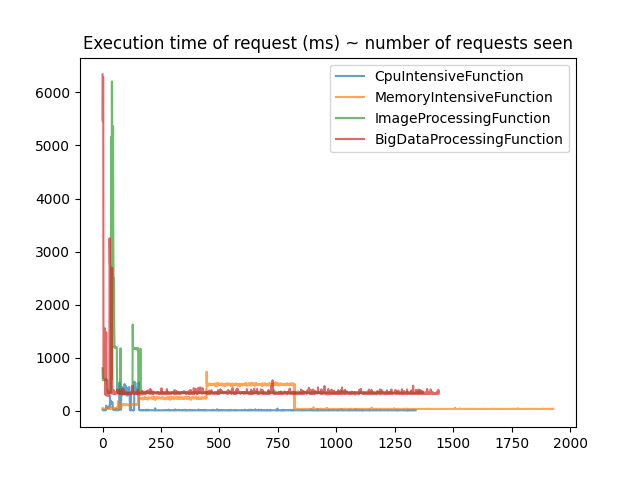
\includegraphics[width=1\linewidth]{images/H1_ExecutionTimeVsNumberOfRequests.PNG}
    \caption{Hypothesis 1: Number of requests needed to reach optimal execution time}
    \label{fig: h1_results}
\end{figure}

\begin{table}
\centering

\begin{tabular}{|p{1in}|p{1in}|p{1in}|}
\hline
Function Type & \# requests to convergence& \# rounds of recommendations to convergence\\
\hline

\hline
CPU-intensive & About 150 & 6\\
\hline
Memory-intensive & About 800 & 9\\
\hline
Image processing & About 170 & 7 \\
\hline
Big data processing & About 50 & 7\\
\hline

\end{tabular}
\caption{Hypothesis 1: Number of requests it takes for the target function to converge to optimal value}
\label{table: 2}
\end{table}

\begin{figure}
    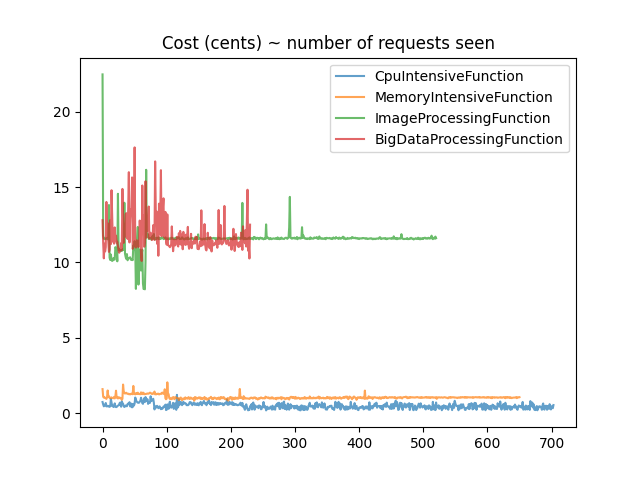
\includegraphics[width=1\linewidth]{images/H1_ExecutionTimeVsNumberOfRequests_Budget.PNG}
    \caption{Hypothesis 1: Number of requests needed to reach optimal cost}
    \label{fig: h1_results_budget}
\end{figure}



%From the baseline data, we will be able to pick the optimal/suboptimal memory size, which serves as the ground truth. We then compare the final memory size that the system converges to with the ground truth, and measure how well does the system successfully find the actual optimal/sub-optimal memory sizes for each FaaS function. Specifically, we plan to measure the percentage of times the system finds the optimal memory size, as well as number of rounds it takes the system to reach a stable memory size recommendation.

\subsection{Hypothesis 2: Optimize Memory Configuration for Execution Time under Varying Workload}

This experiment aims at testing the framework's ability to configure memory to achieve best execution time under varying workload and stable traffic. Here by "varying workload" it means the function receives random input that results in varying amount of computation needed for the function to complete. By "stable traffic" it means the request is sent by load generator in a synchronous manner, the next request is sent only after the previous one is complete.

Fig \ref{fig: h2_results} show the test results. The execution time of each function eventually come down to the lowest possible for that function, which means the agent is able to consistently recommend the best memory configuration available, within 30 to 90 observed executions of the function. 

\begin{figure}
    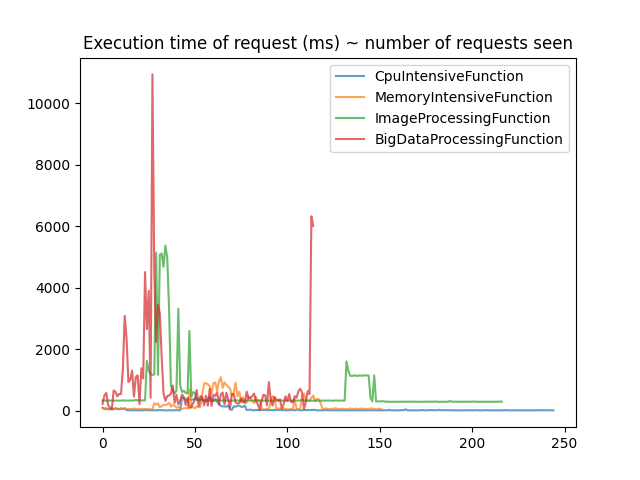
\includegraphics[width=1\linewidth]{images/H2_ExecutionTimeVsNumberOfRequests.png}
    \caption{Hypothesis 2: Number of requests needed to reach optimal performance}
    \label{fig: h2_results}
\end{figure}

Notes and observations from the data:

a. As the model always leaves 10\% chance for exploration, the highest probability of a recommendation that the model would assign is 92\% (90\% + 10\% / 5 options to explore). This is why we are seeing spikes in execution time, as model occasionally tries different memory configuration, and re-assert back to the optimal configuration.

b. The worker updates the memory configuration immediately after a recommendation is made by the agent, but the subsequent request may still get forwarded to the container with previous memory configuration. We suspect that, when the memory configuration is updated, AWS Lambda creates a new container, while the old container still processes the incoming request. And it takes some time before all the traffic is routed to the new container;

c. The cost function on for the image processing function has to be adjusted to 3000 / duration, while it's 1000 / duration for the other three functions. We also tried using (- duration) as cost function, and the agent could not make the expected recommendation. We suspect that the "cost" has to be normalized, which is not well documented for the VowpalWabbit model.

\subsection{Hypothesis 3: Dynamically optimize memory under varying independent workloads}

To measure our framework's ability to dynamically determine optimal memory configuration given changing request patterns, synthetic requests sent out by the traffic modeler were configured to have very different patterns throughout the day, categorized into several cohorts. For instance, one cohort would have a large size of requests, potentially demanding a lambda with higher memory size to support it, while another cohort would consist of lightweight requests.

The workload for this hypotheses were configured similarly to Hypotheses 2, we used randomly varying requests payloads, to simulate varying requests being sent to the functions. However, for this experiment the requests were sent in an asynchronous mode by the load generator, after each request is sent to the function the load generator will not wait for the response before sending the next request, however there was still a small amount of time used for sleeping before sending the next request (0.1 seconds). This simulated independent clients using the function concurrently, pushing the FaaS framework to handle the scheduling of the lambda execution.

The optimization goal for this experiment was duration of requests, also similar to hypotheses 1 \& 2, and the collection of the test results was done in the same way. We analyze the data for convergence to the optimal memory configuration.

Fig. \ref{fig: h3_results} shows the duration time of requests vs the number of requests, for this hypotheses the agent was able to converge on the optimal configuration by the 48th request, however the asynchronous and random payloads of the requests being handled did not significantly improve performance for the Image Processing and the Big Data function (both are high CPU and high memory usage functions).

\begin{figure}
    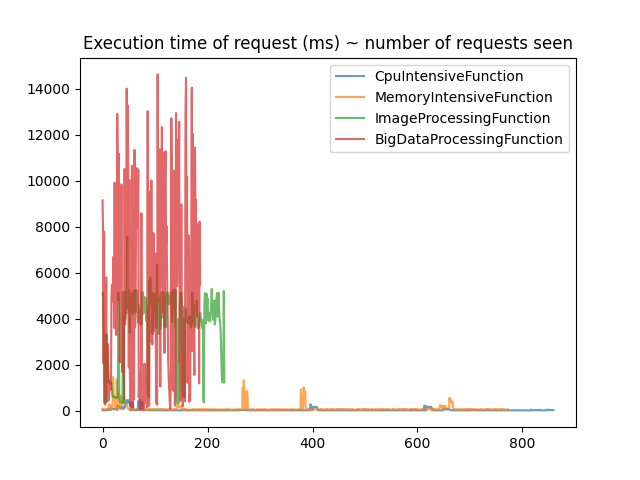
\includegraphics[width=1\linewidth]{images/H3_ExecutionTimeVsNumberOfRequests.png}
    \caption{Hypothesis 3: Number of requests needed to reach optimal performance}
    \label{fig: h3_results}
\end{figure}


\subsection{Hypothesis 4: Adherence to SLO and Optimize for cost}

This experiment expands on hypothesis 3, and the workloads will be similar, asynchronous request with random  payloads. However, the framework will be trying to comply to SLO requirements defined for each of the functions, as well as minimizing monetary cost.

Firstly, we will define an SLO requirement for each function as a request duration time, for this we will use the benchmark results we had initially gathered, and define the 90th percentile of the request duration as the SLO requirement for said function. Before the experiment, we also determined the optimal memory configuration for lowering monetary cost by calculating the average cost of each function at each memory configuration.

Fig \ref{fig: h4_results} show the execution time vs the number of request observed by the the agent. As the figure shows, half of the execution fails to meet the SLO requirement. After around 100 observations, and exploring all configuration options, the agent converged on memory configuration of 128 MB, under which the function neither satisfy the execution time requirement, nor optimizing for cost. Further observations and explorations is not able to changes the agent probability output.

We suspect that the reason for this failure is the reward/cost functions we tried did not yield difference between different configuration, and thus the agent is not able to pick the proper configuration.
\begin{figure}
    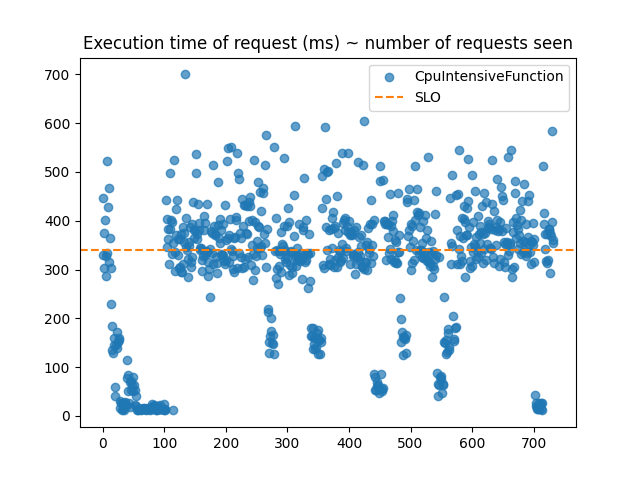
\includegraphics[width=1\linewidth]{images/H4_ExecutionTimeVsNumberOfRequests.png}
    \caption{Hypothesis 3: Number of requests needed to reach optimal performance}
    \label{fig: h4_results}
\end{figure}


%Given other objectives, e.g., cost, we will also collect cost for each request, and measure against baseline cost to understand the system's ability to optimize cost while adhering to SLO.

\section{Discussion}

The first two experiments validate the framework's ability to converge to the ideal memory size that optimizes for simple objective, such as time or budget. The agent starts with exploring different arms, and quickly learns from the early observations to pick the right arm. There are several factors that contributes to the time to convergence: 
\begin{itemize}
    \item frequency of updates of the underlying CMAB agent. The more frequent the agent updates the lambda function, the more quickly the framework is able to explore all candidate arms and start to converge.
    \item Scale of the reward difference between different arms. We observed that for synthetic applications where different memory sizes produce similar performances, it takes longer for the framework to converge, as it spends more time oscillating between arms. The underlying model likely treats the small difference in rewards as noise, and needs more exploration to identify the true winner.
\end{itemize}



In the 4 hypothesis tested in this research, the first one uses constant payload, and the other three uses random payload. Looking at the data, we realize that payload and function type are the main contributor to the varying cost and execution time. Therefore, future research should center around configuring memory according to function type and payload.

There are several system design and experiment setup improvement that couldn't be implemented due to time constraint of this research. The load generator is designed to generate load in different frequency (request per second), however our system is not able to capture this feature and therefore CMAB agent could not use it as an input feature. Note that, by default (and configurable), AWS Lambda can scale up to 1000 container to support parallel execution of requests \cite{Lambda_function_scaling}, thus we suspect that the frequency of the request does not have much impact on the duration of individual executions.

We also observe significant delays in updating the memory configuration of the Lambda function, during which requests will be routed to existing container with previous recommended configuration. This is not a significant issue for the agent as it can still observe accurate execution data, but ideally the system should be able to have request executed on containers with immediate recommended configuration. In future work, we can deploy the same function with different configuration, and have the system route request to these functions accordingly.

\section{Future Work}

\subsubsection{CMAB Optimizations}

CMAB agent optimizations and/or enhancements, based on the outcomes from our experiments, there can be various modifications we can make to the CMAB agent.

Full testing of the CMAB agent is pending, as part of our experiments we plan on making optimizations based on the learnings from our experiments. Thus, the CMAB agent may require further optimization.

The CMAB agent is a core component of our system. Our current design has the CMAB agent running as a lambda function, however we may change this implementation to have it run on our system, if required because of performance and/or resources requirements. The need to run different experiments will require us to have the CMAB agent be available and ready to run, as needed, the current setup as an AWS lambda function should allow for this, however if we need to have a long-lived AWS lambda function then this approach will need to be reconsidered.

The optimizations to the CMAB agent will at least require further work on the agent. But it may also trigger further work on other components. For example, the configuration updater could be changed further to optimize with a new setting (e.g. availability zone, not currently supported).

Although Vowpalwabbit is easy to adopt, it limits the framework's ability to more flexibly configure the MAB algorithm. For instance, it only provides several simple exploration algorithm like epsilon-greedy, and the exploit algorithm in its backend is restricted to generalized linear regression. This introduces difficulty when we want to explore more dynamically, and when we want to have a look-back window to only look at performance of recent executions. It is worth exploring other multi-armed bandit algorithms and implementations in addition to the linear-regression based Vowpalwabbit. Thompson Sampling with Laplace approximation could be a better option.

\subsubsection{System Improvement}

Following the the discussion section, these system improvement can be made. The synthetic functions should be deployed separately with all the different memory configuration options. The Configuration updater should be replaced by a request router that routes requests according to the payload size.  The Load generator should have control over the payload size, the experiments can be designed to evaluate how payload impact the optimization goal.

\section{Conclusion}

Adopting serverless function for latency and cost sensitive application introduces significant resource configuration challenge. To address this challenge, we design and evaluate a system that uses contextual multi-armed bandit (CMAB) agent to recommend and update resource configuration of serverless functions. The system was trained and tested on four different types of functions deployed on AWS Lambda. While the system was able to learn and adapt quickly when given single optimization goals, it fails to optimize for more complex goal, i.e. optimize for cost while satisfying SLO (execution time limit). Future improvement on the agent and the system is needed to better address the challenge of resource configuration for serverless functions.


\section{Conferences for Submission}

These are some of the conferences that we could submit our paper. If we wanted to pursue the submission of this paper, we would need to potentially update our system to implement some of the improvements mentioned, and hopefuly get better results from our system.

\begin{enumerate}
    \item IEEE CLOUD 2024 - In the call for papers there are relevant topics to our paper, specifically the Function as a Service subtopic. Submission deadline is still not posted. The conference should be in the Summer 2024.
    \item EuroSys 2024 - This conference has two paper areas which are relevant to our paper, Cloud computing and machine learning for systems. The conference is Summer 2024.
    \item IEEE Cloud Summit 2024 - This conference has two subtopics which are a match to our paper, Serverless Computing and Machine Learning. The conference is schedued for the Summer 2024.
    \item IEE BCD 2024 - This conference has the topic Cloud Optimization and Automation in which we could submit our paper. The conference is the Summer 2024.
    \item Middleware 2024 - One of the conference's main topic is the Cloud, and it is a place where you can find many research papers on FaaS. The conference is Fall 2024.
    \item IEEE/ACM CCGRID 2025 - Conference on cloud is relevant to our paper. Submission deadlines would be Fall 2024, conference would be in Sprint 2025.
\end{enumerate}

\bibliographystyle{IEEEtran}
\bibliography{refs}

\end{document}
